\section{Results: A Consistent Gain from History}
\label{sec:results-gain}

In this section, we show that history lowers the error of the best model in every study and setting. Section~\ref{subsec:error-levels} sets out the error levels of the three studies; Sections~\ref{subsec:gain-grid}--\ref{subsec:gain-macro} then present the gain in the controlled grid, the $25\times25$ runs and the macro cell, and Section~\ref{subsec:robustness} tests it under changed propagation, a blocked line of sight and no interfering BSs.

\subsection{Error Levels Across the Studies}
\label{subsec:error-levels}

% src: paper/tables/T2_cross_study.md (grid and 25x25 rows; grid: trees single run, CNN/GRU three seeds; 25x25: GRU h=15 three seeds, others single run; 25x25 errors are 3D); macro rows: followup_2026_10/uniform_nlos/history_mechanism_followup_summary.json summary.{xgboost,random_forest}.{snap,full}.{multi,single}.mae_by_stratum.all (20 seeds: XGB 18.74/15.59 multi, 36.33/36.51 single; RF 18.76/16.01 multi, 36.80/36.38 single); naive_baseline/uniform_nlos (20 seeds: multi 35.27, single 38.50)
The three studies operate at very different error scales, and the history gain is therefore measured in each against its own reference. Table~\ref{tab:cross-study} lists, for every setting, the error of the best model without history, the error of the best model with history, and the error of always predicting the mean training position. History lowers the error of the best model in every row but one: single-antenna devices in the macro cell, which are also the only row in which the snapshot model is barely better than the constant guess. Section~\ref{sec:results-no-gain} examines that row.

\begin{table}[h]
  \centering
  \caption{Mean position error~(m) of the best model without and with history, against a constant guess of the mean training position.}
  \label{tab:cross-study}
  \small
  \begin{tabular}{@{}lllccc@{}}
    \toprule
    Study & Setting & AoA & Best snapshot & Best with history & Constant guess \\
    \midrule
    $15\times15$ grid, mixed & BS at center & no & $5.21$ & $1.24$ & $10.9$ \\
     & BS at center & yes & $1.25$ & $0.60$ & $10.9$ \\
     & BS beyond corner & no & $4.93$ & $1.42$ & $10.9$ \\
     & BS beyond corner & yes & $4.25$ & $1.30$ & $10.9$ \\
    \midrule
    $25\times25$ regression & UMi LOS & no & $14.5$ & $12.4$ & $37.3$ \\
     & UMi LOS & yes & $8.2$ & $6.6$ & $37.3$ \\
     & uniform NLOS & no & $29.3$ & $16.7$ & $37.3$ \\
     & uniform NLOS & yes & $16.0$ & $8.0$ & $37.3$ \\
     & mixed & no & $24.3$ & $16.7$ & $37.3$ \\
     & mixed & yes & $13.3$ & $8.7$ & $37.3$ \\
    \midrule
    Macro cell, uniform NLOS & multi-antenna & yes & $18.7$ & $15.6$ & $35.3$ \\
     & single-antenna & no & $36.3$ & $36.4$ & $38.5$ \\
    \bottomrule
  \end{tabular}
\end{table}

% src: CLAIM_EVIDENCE_MAP.md C7 (identity; tests src/python/tests/test_error_metrics.py, error_audit_grid.py); FINAL_REPORT.md §7.5 (784 vs 9,216 m^2; ~1,600 vs 178 samples per cell); pathloss_fit_summary.json (gamma 3.264, sigma 10.106 dB; sigma_r 67.94 m at 95 m, 7.13 m at 10 m)
The errors of the macro cell are not those of the grid. For a classifier, the mean error $\bar{e}$ and the exact-cell accuracy $a$ are tied by
\begin{equation}
  \bar{e} = (1-a)\,\bar{d}_{\text{wrong}},
  \label{eq:mae-accuracy}
\end{equation}
where $\bar{d}_{\text{wrong}}$ is the mean distance between the true cell and a wrong prediction; on a \qtyproduct{28 x 28}{\meter} grid an accuracy of about \SI{60}{\percent} therefore implies an error of a few meters. The errors of tens of meters belong to the macro cell, which covers twelve times the area, offers about nine times fewer training samples per cell, and tests on users the model has never seen. The distance also changes what a single report says about range. Fitting Equation~(\ref{eq:path-loss}) to all macro-cell snapshots gives $\gamma = 3.26$ and a shadowing spread of $\sigma = \SI{10.1}{\decibel}$, and dividing $\sigma$ by the gradient of Equation~(\ref{eq:rss-gradient}) gives the range uncertainty of one RSS reading: \SI{68}{\meter} at the median macro-cell range of \SI{95}{\meter}, against \SI{7}{\meter} at the \SI{10}{\meter} typical of the controlled grid. For additional details on the macro-cell error distribution, we refer the reader to Appendix~\ref{app:macro-errors}.

\subsection{The Controlled Grid}
\label{subsec:gain-grid}

% src: docs/results_of_record/controlled_grid_2026_10/comparison_sets.md (XGB no-AoA history gain +13.2..+27.4 pp, +2.55..+4.29 m; RF +4.9..+13.0 pp, +0.96..+3.06 m; with AoA MAE lower in 12/12; XGB BASE_H3 centre: NLOS 29.6, RMa 50.6, mixed 59.1 %); technical_documentation_revised.md 6.1
The controlled grid was simulated under three propagation settings, each with the BS at the grid center and beyond its corner. The mixed setting is the reference set, because it is the only one in which the propagation changes along a walk; the other two bracket it. Without AoA, adding three steps of history to RSS and SINR raised exact-cell accuracy in all twelve configurations of setting, placement and classifier~(Figure~\ref{fig:cg-sets} in Appendix~\ref{app:grid-accuracy}) and lowered the mean error in all twelve, by $2.6$ to \SI{4.3}{\meter} for XGBoost and by $1.0$ to \SI{3.1}{\meter} for Random Forest~(Figure~\ref{fig:grid-mae}); with AoA, history lowered the mean error in all twelve as well. The absolute accuracy, in contrast, moves by tens of points with the propagation: with the BS at the center, XGBoost with history reaches \SI{30}{\percent} under uniform NLOS and \SI{59}{\percent} under the mixed setting. Part of XGBoost's larger gain is recovery from a weak snapshot model, but both classifiers gain in every set.


\begin{figure}[b]
  \centering
  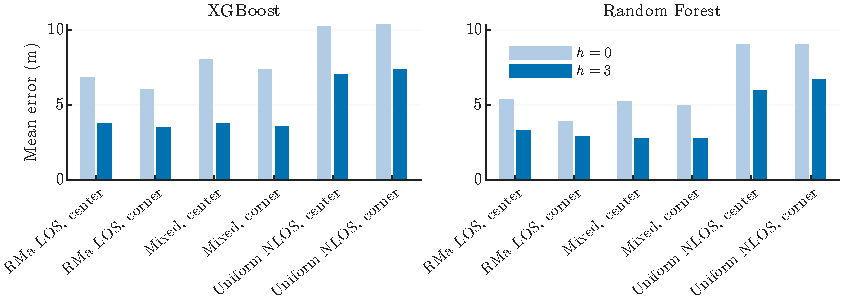
\includegraphics[width=0.95\textwidth]{fig_grid_mae}
  \caption{Controlled grid: mean position error from RSS and SINR at $h=0$ and $h=3$, per classifier, propagation setting and BS placement. Single run per bar.}
  \label{fig:grid-mae}
\end{figure}
% src: figure_scripts/fig_grid_mae.m (MATLAB); data/grid_comparison_sets.csv (= controlled_grid_2026_10/comparison_sets.csv)

% src: comparison_sets.csv (aoa_gain_pp BASE_H3 -> BASE_A_H3, XGBoost: centre 20.9 / 19.5 / 38.5; NE 4.0 / 1.0 / 6.2; history gain with AoA in m: centre 0.21-0.61, NE 0.74-2.03); results_summary.csv of centre_bs_mixed_30 (device parameters: XGB 59.2 -> 66.7 %, RF 65.7 -> 71.8 %)
The BS placement decides how much the angle is worth, whereas history helps at both placements. With history already in the input, adding AoA raised XGBoost's accuracy by $19.5$ to $38.5$ points with the BS at the center but by only $1.0$ to $6.2$ points beyond the corner, from where the whole grid falls within a wedge of about \ang{52} that a \ang{5} codebook barely resolves. Correspondingly, with AoA available, history lowers the error more beyond the corner~($0.7$ to \SI{2.0}{\meter}) than at the center~($0.2$ to \SI{0.6}{\meter}), where the angle already leaves little error to remove. Because RSS and SINR are stacked in absolute form, history could also be helping only by identifying the device; however, supplying the device parameters directly leaves a history gain of $6$ to $8$ points on top of them.

\subsection{The $25\times25$ Regression Runs}
\label{subsec:gain-regression}

% src: docs/results_of_record/regression_25x25_2026_10/{umilos,nlos,mixed}_30_fixednoise/{tuned,segment_shuffle}/results_summary.csv and sequence_vs_trees/all_mae.md (UMi LOS RF 14.52 -> 17.06, shuffled 14.73 -> 18.32; XGB 29.39 -> 13.72; NLOS XGB 33.25 -> 24.51, RF 29.32 -> 26.61; mixed XGB 29.89 -> 20.46, RF 24.33 -> 23.19); features_test (RF hybrid 8.14 vs 8.85; mixed 11.96 vs 11.75)
The $25\times25$ regression runs, which pool five simulated device profiles and test on the later part of each walk, show the same result at the macro-cell geometry~(Figure~\ref{fig:single-user}): without an angle, the best model with history beats the best snapshot model under all three propagation settings, and with the GRU of Section~\ref{sec:results-window} it does so with an angle as well~(Table~\ref{tab:cross-study}). The gain is not universal across models. On UMi LOS data Random Forest's error rose with three steps of history, under a chronological split and when the walk was cut into shuffled five-step blocks to prevent memorization of the path, while XGBoost's fell sharply from a snapshot model about twice as poor.\footnote{Replacing the stacked absolute lags with differences from the current snapshot removed Random Forest's loss in a related configuration with AoA, which points to its feature subsampling as the cause, but did not help on the mixed set.} Under uniform NLOS and mixed propagation both ensembles gain.

\begin{figure}[t]
  \centering
  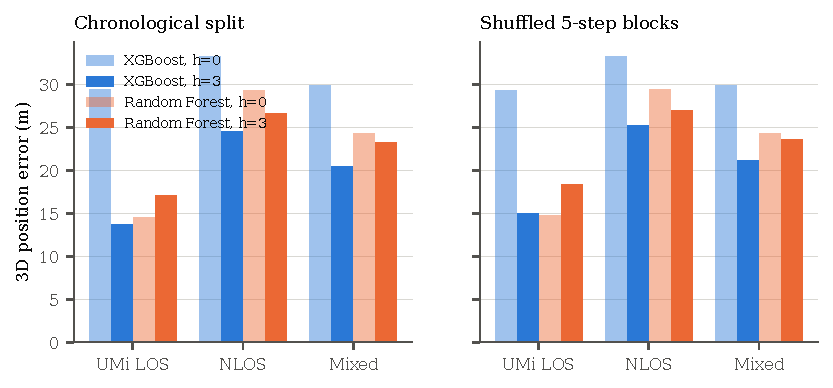
\includegraphics[width=0.85\textwidth]{fig_regression25_no_aoa}
  \caption{$25\times25$ regression with RSS and SINR only: mean position error at $h=0$ and $h=3$ for XGBoost and Random Forest, under a chronological and a block-shuffled split. Single run per bar; the shuffled split cuts each walk into five-step blocks.}
  \label{fig:single-user}
\end{figure}
% src: figure_scripts/python/make_figures_followup.py regression25_no_aoa(); docs/results_of_record/regression_25x25_2026_10

\subsection{The Macro Cell}
\label{subsec:gain-macro}

% src: data/seed_repeats_uniform_nlos.json (five splits; k-NN, GRU, 1D-CNN, mask-aware 1D-CNN, 1D-CNN + attention) and data/followup20_uniform_nlos.json (20 splits; XGBoost, RF); recomputed by figure_scripts/fig_history_gain_ci.m: multi-antenna gains 2.75 (RF) to 4.06 m (attention), 14.6-20.8 %; all Student-t intervals clear of zero
For multi-antenna devices in the macro cell, history lowered the error of every one of the seven model families, by $2.8$ to \SI{4.1}{\meter}, or $15$ to \SI{21}{\percent} of each model's own $h=0$ error~(Figure~\ref{fig:history-gain-ci}; per-model values in Table~\ref{tab:history-gain}). Every interval is clear of zero. The gain is of similar size across instance-based, bagged, boosted, recurrent, convolutional and attention-based models, so it comes from information that the $h=0$ input lacks and does not depend on the inductive bias of one architecture. These gains are measured under the angle impairment of Section~\ref{subsec:device-model}, in which every report carries an independent \ang{4} error; Section~\ref{subsec:averaging} examines how much of the gain depends on this independence.

\begin{figure}[t]
  \centering
  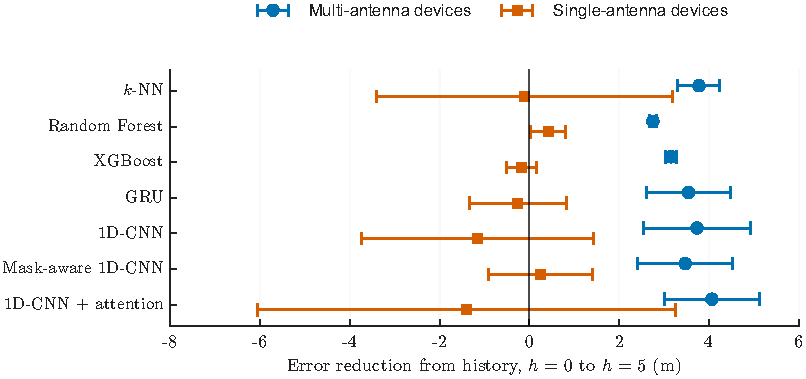
\includegraphics[width=0.8\textwidth]{fig_history_gain_ci}
  \caption{Macro cell, uniform NLOS: reduction in mean error from $h=0$ to $h=5$ per model and device group. Seed-paired means with \SI{95}{\percent} Student-$t$ intervals over $20$ user splits~(XGBoost, Random Forest) or five~(other models).}
  \label{fig:history-gain-ci}
\end{figure}
% src: figure_scripts/fig_history_gain_ci.m (MATLAB); data/seed_repeats_uniform_nlos.json, data/followup20_uniform_nlos.json

% src: data/macro_uniform_nlos_errors_seed42.csv (from diagnostics_2026_10/baseline_uniform_nlos/errors_first_seed.npz, seed 42) via figure_scripts/fig_macro_error_map.m: XGBoost multi 18.99 -> 15.41 m, single 34.66 -> 34.71 m; per-grid-point means: history lowers the multi-antenna error at 83 % of points (single 44 %); single-antenna h=5 error 22.6 m within 20 m of the area centre, 50.5 m beyond 40 m
Figure~\ref{fig:macro-error-map} shows where the errors fall. For multi-antenna devices the error is spread fairly evenly over the area, and history lowers it at \SI{83}{\percent} of the grid points. For single-antenna devices the error is lowest around the middle of the area and largest along its edges, with or without history, which is the pattern expected of predictions drawn toward the mean position.

\begin{figure}[t]
  \centering
  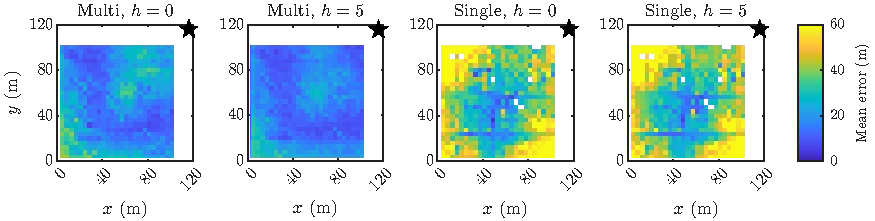
\includegraphics[width=\textwidth]{fig_macro_error_map}
  \caption{Macro cell, uniform NLOS: mean position error per grid point, XGBoost at $h=0$ and $h=5$, per device group, one user split. The star marks the serving BS.}
  \label{fig:macro-error-map}
\end{figure}
% src: figure_scripts/fig_macro_error_map.m (MATLAB); data/macro_uniform_nlos_errors_seed42.csv

% src: seed_repeats_all_models_summary.json ranking (h=5 overall, ranks 1-6 18.810-19.275); master_benchmark_rerun_summary.json (XGBoost 4 s training); xgb_per_h_retune_summary.json, rf_per_h_retune_summary.json (XGBoost tuning <= 0.44 m; RF < 0.07 m); followup_2026_10/history_depth (XGB full +1.21, +2.53, +3.15, +3.51, +3.68 at h = 1, 3, 5, 10, 20; 10-20 seeds); rts_retune_all_models_summary.json (RTS 2.5-4.7 %, test-tuned, backward pass)
With history in place, the choice of model matters far less than the input. At $h=5$ the six trained models other than $k$-NN fall within \SI{0.47}{\meter} of each other in overall error, and XGBoost reaches that level in \SI{4}{\second} of training. Re-tuning XGBoost and Random Forest separately at every depth, on training users only, changed their errors by at most \SI{0.44}{\meter} and left the history gain essentially unchanged~(Table~\ref{tab:supp-retune}), so the gain does not depend on hyperparameters chosen for one input size. The gain builds over the first steps of history~(Figure~\ref{fig:history-by-group} in Appendix~\ref{app:supplementary}): for XGBoost one extra report is worth \SI{1.2}{\meter}, and most of the gain is in place by ten.

\subsection{Propagation, Blockage and Interference}
\label{subsec:robustness}

% src: data/seed_repeats_mixed.json and data/followup20_mixed.json via figure_scripts/fig_history_gain_ci.m (multi-antenna gains 2.36 (RF) to 3.89 m, all intervals clear of zero; single-antenna XGB +1.14 +- 0.29, RF +1.28 +- 0.37, others span zero); seed_repeats ranking h=5 16.98-17.34 for ranks 1-6
\noindent\textbf{Mixed LOS and NLOS propagation.} Giving the four regions of the macro cell their own LOS or NLOS propagation leaves the multi-antenna result intact~(Figure~\ref{fig:mixed-gain}). History lowered the error of all seven families, by $2.4$ to \SI{3.9}{\meter}, and the six trained models other than $k$-NN again lie within \SI{0.4}{\meter} of each other. The single-antenna result differs from that of uniform NLOS, since both tree ensembles now gain $1.1$ to \SI{1.3}{\meter}; Section~\ref{subsec:mixed-single} examines where that gain arises. History also helps more in the regions that carry LOS propagation, but the same regions show the same difference in the uniform-NLOS realization, which contains no LOS at all; the difference is therefore a property of the regions, which lie in the range bands with the most error to remove, and not of LOS propagation~(Appendix~\ref{app:propagation}).
% src: followup_2026_10/mixed_propagation/region_gain_did_vs_uniform.json (20 seeds: gap 1.81 +- 0.27 uniform vs 1.54 +- 0.24 mixed; difference -0.27 +- 0.25; RF -0.01 +- 0.18)

\begin{figure}[t]
  \centering
  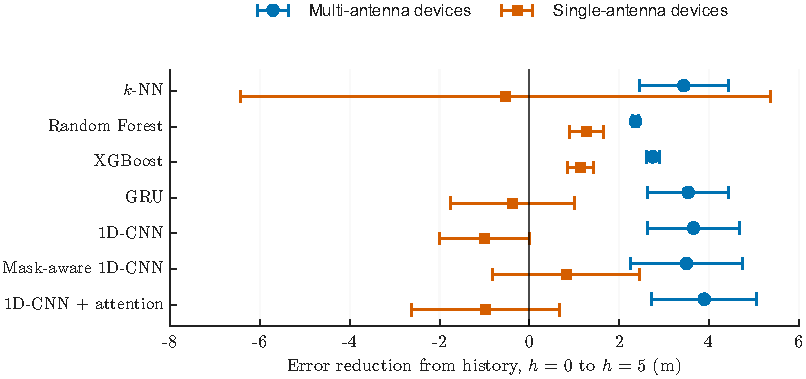
\includegraphics[width=0.8\textwidth]{fig_mixed_history_gain_ci}
  \caption{Macro cell, mixed propagation: reduction in mean error from $h=0$ to $h=5$ per model and device group. Seed-paired means with \SI{95}{\percent} Student-$t$ intervals over $20$ user splits~(XGBoost, Random Forest) or five~(other models).}
  \label{fig:mixed-gain}
\end{figure}
% src: figure_scripts/fig_history_gain_ci.m (MATLAB); data/seed_repeats_mixed.json, data/followup20_mixed.json

% src: CONTINUE_HERE.md §4 (prediction); followup_2026_10/blocked_los/history_mechanism_followup_summary.json (20 seeds, 360 users; multi-antenna XGBoost: blocked +6.29 +- 0.18 m (36.1 %), unblocked +6.66 +- 0.15 (38.7 %); by width +5.24 .. +6.11 m for 5-120 m, +7.65 m at 150 m; angle_mean blocked +6.51 +- 0.18; single-antenna blocked +0.47 +- 0.54)
% src: configs/b6_los_blocked_los_config.jsonc (corridor length 200 m; strip widths 5-150 m; speeds 1.5, 4.0, 10.0 m/s; BS [100,500,10]; UMi LOS / UMi NLOS); CONTINUE_HERE.md §4 (360 users, constant-range rationale)
\noindent\textbf{A blocked line of sight.} The fourth deployment follows UEs walking a straight \SI{200}{\meter} corridor whose middle section passes behind an obstruction, so that the link goes from LOS to NLOS and back; the width of the blocked strip varies from $5$ to \SI{150}{\meter}, and the BS stands \SI{500}{\meter} from the corridor so that the range is nearly constant along it. The scenario was designed to test whether history becomes more valuable as a blockage lengthens, up to the point where the heading observed before the blockage stops being informative. Over $20$ splits, history lowered the error of multi-antenna devices by \SI{36}{\percent} inside the blocked stretch and by \SI{39}{\percent} outside it for XGBoost, and the reduction does not rise and fall with the width of the blocked strip~(Figure~\ref{fig:blocked}), so the predicted dependence on blockage length does not appear. At that distance an azimuth step of \ang{5} spans tens of meters, and the unordered mean of the angle window recovers all of the gain, as in the macro cell. History thus keeps its value through a blockage of every length tested. Single-antenna devices gain nothing detectable in this scenario, inside or outside the blocked stretch.

\begin{figure}[h]
  \centering
  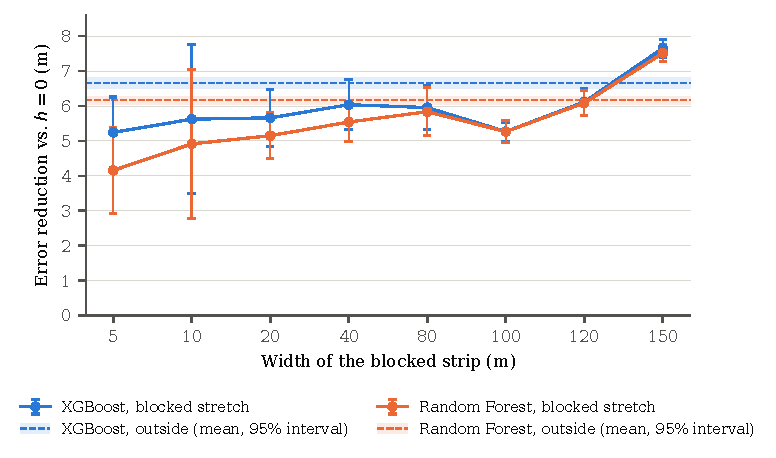
\includegraphics[width=0.7\textwidth]{fig_blocked_by_width}
  \caption{Blocked line of sight: reduction in multi-antenna error from $h=0$ to $h=5$ inside the blocked stretch, by strip width, with the mean outside it as a band. Seed-paired means over $20$ user splits with \SI{95}{\percent} Student-$t$ intervals.}
  \label{fig:blocked}
\end{figure}
% src: figure_scripts/python/make_figures_followup.py blocked_by_width()

% src: followup_2026_10/no_interference/{uniform_nlos,mixed_propagation}/history_mechanism_followup_summary.json (20 seeds; median SINR -3.0 dB; multi-antenna gain larger without interferers by 0.29-0.44 m; single mixed XGB 1.04 +- 0.23 vs 1.14 +- 0.29)
\noindent\textbf{Without the interfering BSs.} Both macro-cell realizations are interference-limited, with a median SINR of \SI{-3}{\decibel}. Switching the interferers off amounts to replacing SINR by the signal-to-noise ratio computed from the stored RSS. Over $20$ splits the multi-antenna history gain is slightly larger without them, by $0.3$ to \SI{0.4}{\meter}, and the single-antenna gain under mixed propagation is unchanged~(Table~\ref{tab:no-interference}); the conclusions do not depend on the interferers.
